% -*- TeX -*- -*- Soft -*-
\documentclass[article,shortnames,nojss]{jss}

%\VignetteIndexEntry{Transformations in regression with fsdaR}
%\VignetteKeywords{robustness, multivariate analysis, MCD, R, statistical design patterns}
%\VignettePackage{fsdaR}

\usepackage{float}
\floatplacement{figure}{H}

\usepackage{amsmath}                %% need for subequations
\usepackage{amssymb}
\usepackage{amsfonts}
\usepackage[english]{babel}

%%%%%%%%%%%%%%%%%%%%%%%%%%%%%%
%% declarations for jss.cls %%%%%%%%%%%%%%%%%%%%%%%%%%%%%%%%%%%%%%%%%%
%%%%%%%%%%%%%%%%%%%%%%%%%%%%%%
\newcommand{\vv}[1]{\mbox{\boldmath$#1$}}
\newcommand{\xv}{\mbox{\boldmath$x$}}
\newcommand{\yv}{\mbox{\boldmath$y$}}
\newcommand{\zv}{\mbox{\boldmath$z$}}
\newcommand{\mv}{\mbox{\boldmath$m$}}
\newcommand{\tv}{\mbox{\boldmath$t$}}
\newcommand{\xbarv}{\mbox{\boldmath$\bar x$}}
\newcommand{\uv}{\mbox{\boldmath$u$}}
\newcommand{\muv}{\mbox{\boldmath$\mu$}}
\newcommand{\nuv}{\mbox{\boldmath$\nu$}}
\newcommand{\deltav}{\mbox{\boldmath$\delta$}}
\newcommand{\chiv}{\mbox{\boldmath$\chi$}}
\newcommand{\ov}{\mbox{\boldmath$0$}}

\newcommand\MCD{\mathit{MCD}}
\newcommand\MVE{\mathit{MVE}}
\newcommand\OGK{\mathit{OGK}}
\newcommand\diag{\mathrm{diag}}
%\newcommand\det{\mathrm{det}}

\newcommand{\class}[1]{``\code{#1}''}
\newcommand{\fct}[1]{\code{#1()}}

%% almost as usual
\author{The FSDA Team}
\title{Transformations in regression with fsdaR}

%% an abstract and keywords
\Abstract{
\noindent Several analyses of regression data sets can be improved by using a transformation of the response, rather than the original response itself. More specifically, the transformation may improve the approximate normality or the homogeneity of the errors. In a lot of examples there are physical reasons why a transformation might be expected to be helpful. For instance if the response is a non negative variable, it cannot be subject to additive errors of constant variance. In this vignette we consider the parametric family of power transformations introduced by Box and Cox (1964).
} \Keywords{transformations, Box-Cox transformation, robustness, outliers}
%% at least one keyword must be supplied

%% The address of (at least) one author should be given
%% in the following format:
\Address{
  Valentin Todorov\\
  UNIDO\\
  Vienna, Austria\\
  E-mail: \email{valentin.todorov@chello.at}\\
}

%% for those who use Sweave please include the following line (with % symbols):
%% need no \usepackage{Sweave.sty}

%% end of declarations %%%%%%%%%%%%%%%%%%%%%%%%%%%%%%%%%%%%%%%%%%%%%%%

\newcommand{\bi}{\begin{itemize}}
\newcommand{\ei}{\end{itemize}}
\newcommand{\be}{\begin{enumerate}}
\newcommand{\ee}{\end{enumerate}}
\renewcommand{\v}[1]{\mathbf{#1}}
%% Sweave options for the complete document
%%\SweaveOpts{keep.source=TRUE}
%%\SweaveOpts{prefix.string=images/oofgen/oof}


\begin{document}


%% include your article here, just as usual
%% Note that you should use the \pkg{}, \proglang{} and \code{} commands.

\section[Introduction]{Introduction}
%% Note: If there is markup in \(sub)section, then it has to be escape as above.
Several analyses of regression data sets can be improved by using a transformation of the response, rather than the original response itself. More specifically, the transformation may improve the approximate normality or the homogeneity of the errors. In a lot of examples there are physical reasons why a transformation might be expected to be helpful. For instance if the response is a non negative variable, it cannot be subject to additive errors of constant variance.

In this vignette we consider the parametric family of power transformations introduced by \citet{box:1964}. A full discussion can be found in \citet{atkinson:2000}. Given that the estimated transformation and the related test statistics may be sensitive to the presence of one or several outliers, we use the forward search to see how the estimates and statistics evolve as we move through the ordered data. As the user will see, influential observations may only be evident for some transformations of the data. Since observations that appear as outlying in the original (not transformed) data may not be outlying once the data have been transformed, and vice versa, we employ the forward search on the data subject to the various transformations, as well as on the original data.

\section{Score test for transformation}
In this Section we will consider an approximate score test statistic for testing the transformation $\lambda=\lambda_0$.

Box and Cox \citep{box:1964} analyzed the normalized power transformation given by the following equation

\begin{equation}
\label{eq:1}
    z(\lambda)  = \begin{cases}
      (y^\lambda-1)/\lambda \dot{y}^{\lambda-1} & \text{$\lambda \neq 0$}\\
      \dot{y} \log y & \text{$\lambda = 0$}
    \end{cases}
    \tag{1}
\end{equation}

where the symbol $y$ with dot on top denotes the geometric mean of the observations.

When $\lambda=1$, there is no transformation: $\lambda=\frac{1}{2}$ is the square root transformation, $\lambda=0$ gives the\emph{log} transformation and $\lambda=-1$ the reciprocal. These are the most widely used transformations, frequently supported by some empirical reasoning. For example, measurements of concentration often have a standard deviation proportional to the mean, so that the variance of the logged response is approximately constant. For this form of transformation to be applicable, all observations need to be positive. For it to be possible to detect the need for a transformation the ratio of largest to smallest observation should not be too close to one. A similar requirement applies to the transformation of explanatory variables.

The hope is that, for some $\lambda$ which has to be estimated, the transformed observations will satisfy the linear regression model given by the following equation:

\begin{equation}
\label{eq:2}
  z(\lambda) = x^\top \beta + \epsilon
  \tag{2}
\end{equation}

where $x$ is $p\times 1$ and the errors are independently normally distributed with constant variance $\sigma^2$. For inference about the transformation parameter $\lambda$, Box and Cox suggest the likelihood ratio test statistic. For regression models, a computationally simpler alternative test of the hypothesis $\lambda=\lambda_0$ is the approximate score statistic derived by Taylor series expansion of Equation (1) given above.

\begin{equation}
\label{eq:3}
  z(\lambda) = z(\lambda_0) + (\lambda-\lambda_0) \omega(\lambda_0)
  \tag{3}
\end{equation}

where

\[
  \omega(\lambda_0) = \frac{\partial z(\lambda)}{\partial\lambda}
  \bigg\rvert_{\lambda=\lambda_0}
\]

If the linearized response given in Equation (3) is substituted in the regression model (2), the model becomes as shown in Equation (4)

\begin{equation}
\label{eq:4}
  z(\lambda_0) = x^\top \beta - (\lambda-\lambda_0) \omega(\lambda_0) + \epsilon
  \tag{4}
\end{equation}

Because Equation (4) is again a regression model with an extra variable $\omega(\lambda_0)$ derived from the transformation, the new variable is called the constructed variable for the transformation. If the true value of $\lambda$ is close to $\lambda_0$, the coefficient $(\lambda-\lambda_0)$ of the constructed variable will be small. The regression model (4) can be rewritten more conventionally by putting $\gamma=-(\lambda-\lambda_0)$, as shown in Equation (5):

\begin{equation}
\label{eq:5}
  z(\lambda_0) = x^\top \beta + \gamma \omega(\lambda_0) + \epsilon
  \tag{5}
\end{equation}

Small values of $\gamma$ then indicate that no transformation is necessary. The approximate score statistic for testing the transformation $\lambda=\lambda_0$ (which is often denoted in the statistical literature with symbol $Tp(\lambda)$ is just the t-statistic for the coefficient of regression on $\omega(\lambda_0)$ in Equation (5).

\subsection[Example 1: wool data]{Example 1: \code{wool} data}

Compute the score test for the \code{wool} data set:


\begin{Schunk}
\begin{Sinput}
> library(fsdaR)
> data(wool)
> head(wool)
\end{Sinput}
\begin{Soutput}
  length amplitude load cycles
1     -1        -1   -1    674
2     -1        -1    0    370
3     -1        -1    1    292
4     -1         0   -1    338
5     -1         0    0    266
6     -1         0    1    210
\end{Soutput}
\begin{Sinput}
> ##  Compute the score test using the five most common values of the
> ##  transformation parameter lambda
>
> out <- score(cycles~., data=wool)
> out$Score
\end{Sinput}
\begin{Soutput}
   la=-1.00    la=-0.50    la= 0.00    la= 0.50    la= 1.00
 17.7059127   7.4926857  -0.9122373  -9.5511225 -18.5575519
>\end{Soutput}
\begin{Sinput}
>
\end{Sinput}
\end{Schunk}

The constructed variable is not significant when we consider $\lambda=0$.

\subsection[Example 2: loyalty cards data]{Example 2: \code{loyalty cards} data}

Compute the score test for the \code{loyalty cards} data set:


\begin{Schunk}
\begin{Sinput}
> data(loyalty)
> head(loyalty)
\end{Sinput}
\begin{Soutput}
  visits age family amount_spent
1     12  54      4          696
2      4  36      4          309
3      6  65      2          295
4      3  45      3          101
5      3  29      3           71
6      5  54      3          144
\end{Soutput}
\begin{Sinput}
> ## la is a vector containing the values of \lambda which have to be tested
>
> out <- score(amount_spent~., data=loyalty,
+               la=c(0.25, 1/3, 0.4, 0.5))
> out$Score
\end{Sinput}
\begin{Soutput}
   la=0.25    la=0.33    la=0.40    la=0.50
 4.3159860 -0.2123694 -3.8333905 -9.4717057
\end{Soutput}
\begin{Sinput}
>
\end{Sinput}
\end{Schunk}

Using all the observations it seems that the third root is the best value of the transformation parameter.



\section{Forward Score test}

In the search for the best value of the transformation parameter test statistics are more informative than parameter estimates because, if the likelihood is flat, the estimates can vary widely without conveying any useful information about the transformation.

Given that the score test for transformation is not robust to the presence of particular observations we monitor the values of the score test statistic (see function Score) for several values of the transformation parameter $\lambda$ in each step of the forward search.
If the size of the data set is small (i.e. smaller than 100) generally it is enough to consider the five most common values of $\lambda$: $\lambda=(-1, -0.5, 0. 05, 1)$, otherwise a finer grid of values of $\lambda$ may be needed.

The simultaneous forward plot of the score test statistic for several values of the transformation parameter $\lambda$ is known in the literature as \emph{fan plot}. Each search is separate, so that the observations may, and do, enter in different orders in the searches. This plot enables us to appraise in a quantitative way the percentage of observations in agreement with the different values of the transformation parameter.

Let us consider several examples. We begin with the poison data from [@box:1964]. The observations are time to death of animals in a $3 \times 4$ factorial experiment with four observations at each factor combination.

\subsection[Example 1: Original poison data]{Example 1: Original \code{poison} data}

Box and Cox suggested the reciprocal transformation $(\lambda = -1)$ so that death rate, rather than survival time, has a simple structure. Our analysis is based on five values of $\lambda$: \code{(-1, -0.5, 0, 0.5, 1)}. The data are transformed and a starting point is found by {\bf LMS} for each of the five forward searches, which then proceed independently for each $\lambda$ using the transformed data.

Figure~\ref{fig:ex-1} presents the fan plot of the approximate score statistic $T_p(\lambda)$ for each search as the subset size $m$ increases.
The fan plot is generated by the following R code:


\begin{Schunk}
\begin{Sinput}
> ##  Example 1: original poison data
> data(poison)
> head(poison)
\end{Sinput}
\begin{Soutput}
  X1 X2 X3 X4 X5 X6    Y
1  1  0  0  1  0  0 0.31
2  1  0  0  1  0  0 0.45
3  1  0  0  1  0  0 0.46
4  1  0  0  1  0  0 0.43
5  0  1  0  1  0  0 0.36
6  0  1  0  1  0  0 0.29
\end{Soutput}
\begin{Sinput}
> dim(poison)
\end{Sinput}
\begin{Soutput}
[1] 48  7
\end{Soutput}
\begin{Sinput}
> set.seed(10)
> ##  A formula without intercept looks like this: Y~.-1
> out1 <- fsrfan(Y~.-1, data=poison)    # no intercept
> plot(out1, ylim=c(-14, 3))
>
\end{Sinput}
\end{Schunk}

\begin{center}
\begin{figure}[H]
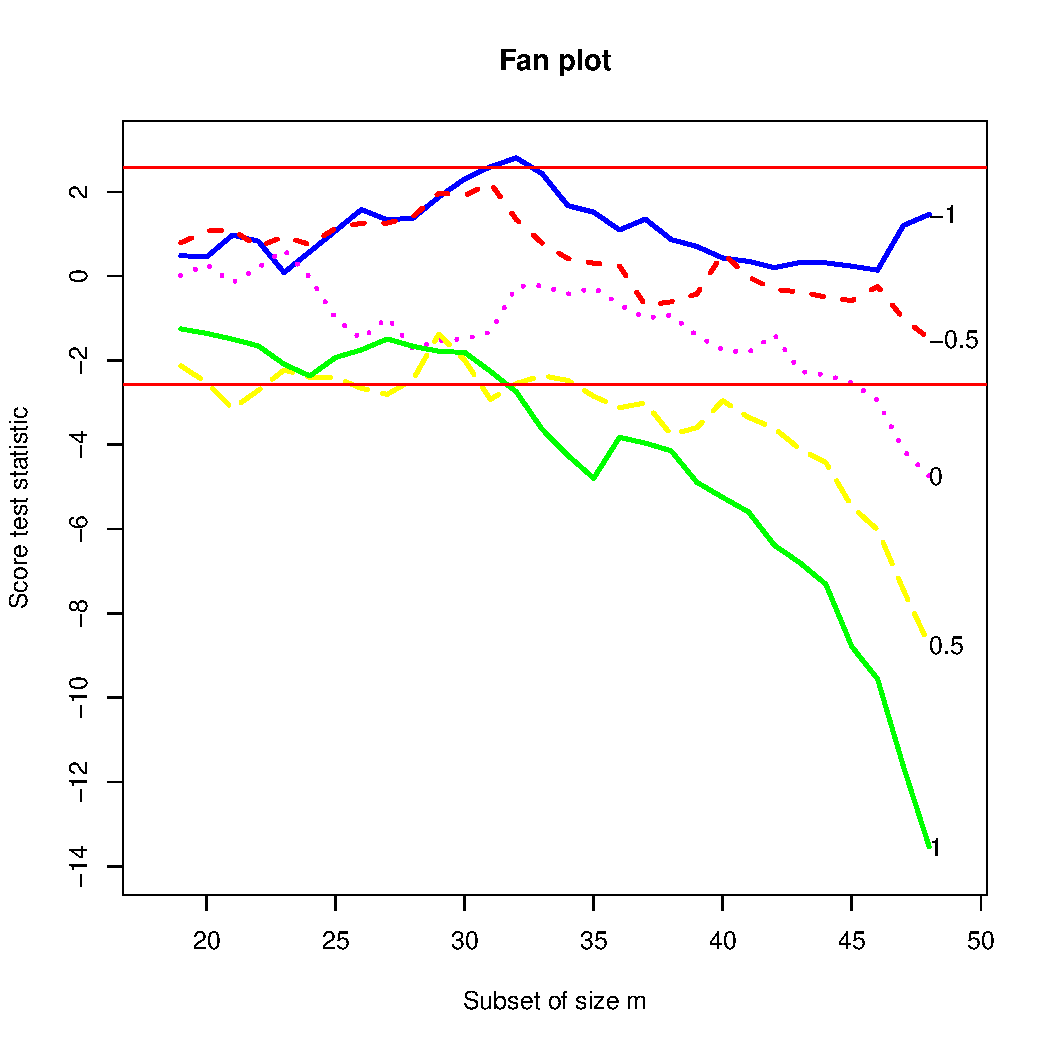
\includegraphics[width=0.8\textwidth]{transreg-ex-1}
\caption{Fan plot for the original \code{poison} data.}
\label{fig:ex-1}
\end{figure}
\end{center}

The central horizontal bands on the figure are at plus or minus 2.58, containing 99\% of a standard normal distribution. For data without outliers, the curves for the different values of $\lambda$ fan out as they do here: if outliers are present, as we will see later in this tutorial, the curves may cross several times. But the final order always has $\lambda=-1$ at the top and $\lambda=1$ at the bottom. Initially, in Figure~\ref{fig:ex-1}, for small subset sizes there is no evidence against any transformation. During the whole forward search there is never any evidence against either $\lambda=-1$ or $\lambda=-0.5$ (for all data the maximum likelihood estimate of $\lambda$ is $-0.75$). The log transformation is also acceptable until the last four observations are included by the forward search. As the table below shows, these include some of the largest observations in order. The plot shows how evidence against the log transformation depends critically on this last 8\% of the data. Evidence that $\lambda$ is different from 1 is spread throughout the data: less than half of the observations are sufficient to indicate the need for some transformation. There are no jumps in this curve, just an increase in evidence against $\lambda=1$ as each observation is introduced into the subset. The relative smoothness of the curves reflects the lack of outliers and exceptionally influential cases.

Now, let us examine the order in which the units enter the subset for the different values of the transformation parameter $\lambda$. For this purpose the three dimensional array \code{Un} returned by \code{fsrfan()} can be used. It consists of \code{length(la)} matrices each with size \code{n-init} by 11. Let us look at the last six observations of \code{Un[,2,]} together with the six observations with largest values of \code{y}, presented in Table~\ref{tab:ex-1}.


% latex table generated in R 4.2.0 by xtable 1.8-4 package
% Sat May  7 21:54:10 2022
\begin{table}[ht]
\centering
\begin{tabular}{rrrrrrr}
  \hline
Step & -1 & -0.5 & 0 & 0.5 & 1 & Largest Obs. \\
  \hline
43 & 27 & 44 & 14 & 43 & 28 & 13 \\
  44 & 28 & 37 & 28 & 28 & 43 & 15 \\
  45 & 37 & 28 & 37 & 14 & 17 & 17 \\
  46 & 44 & 8 & 17 & 17 & 14 & 42 \\
  47 & 11 & 20 & 20 & 42 & 42 & 14 \\
  48 & 8 & 42 & 42 & 20 & 20 & 20 \\
   \hline
\end{tabular}
\caption{The last six observations that enter the model. The last column shows the six largest observations.}
\label{tab:ex-1}
\end{table}

Observation 20 is the largest one. We see in Table~\ref{tab:ex-1} that, for $\lambda=0.5$  and $\lambda=1$, it is the last to enter the model. It enters just before the last $(m = 47)$ in case of $\lambda=0$ and $\lambda=-0.5$ and is not present at all in the last six observations for $\lambda=1$. Similarly, the four largest observations are the last four to enter for $\lambda=1$ and $\lambda=0.5$, but the number decreases as $\lambda$ decreases. For $\lambda=-1$ all six largest observations enter earlier in the search, before $m=43$. However, the next but last observation to enter is 11, which is the smallest one. These results, which are similar to those for the \code{wool} data set shown in the previous Section, are both gratifying and surprising. With a simple sample it is the large observations that would suggest a transformation with $\lambda$ less than one. Since these observations may not be in agreement with the model, they should enter the search for $\lambda=1$ at the end. Likewise, the smallest values would tend to suggest a transformation above the inverse. If a correct transformation has been found, small and large observations should enter the search anytime. They do so here for $\lambda=-0.5$. It is however surprising that these results for a random sample still hold when we fit a linear model to the data.


\subsection[Example 2: Modified poison data (one modified observation)]{Example 2: Modified \code{poison} data (one modified observation)}

For the introduction of a single outlier into the\code{poison} data we follow \citet{andrews:1971} and change observation 8, one of the readings for Poison II, group A, from 0.23 to 0.13. This is not one of the larger observations so the change does not create an outlier in the scale of the original data. The effect on the estimated transformation for all the data is however to replace the reciprocal with the logarithmic transformation: the maximum likelihood estimate of  $\lambda=-0.15$. And, indeed, the fan plot of the score statistics from the forward searches in Figure~\ref{fig:ex-2} below, which can be obtained from the following code, shows that.

\begin{Schunk}
\begin{Sinput}
> ##  Example 2: modified poison data (change y[8] from 0.23 to 0.13)
> library(fsdaR)
> data(poison)
> poison$Y[8] <- 0.13
> set.seed(9999)
> out2 <- fsrfan(Y~.-1, data=poison)
> plot(out2, ylim=c(-11, 9))
\end{Sinput}
\end{Schunk}

\begin{center}
\begin{figure}[H]
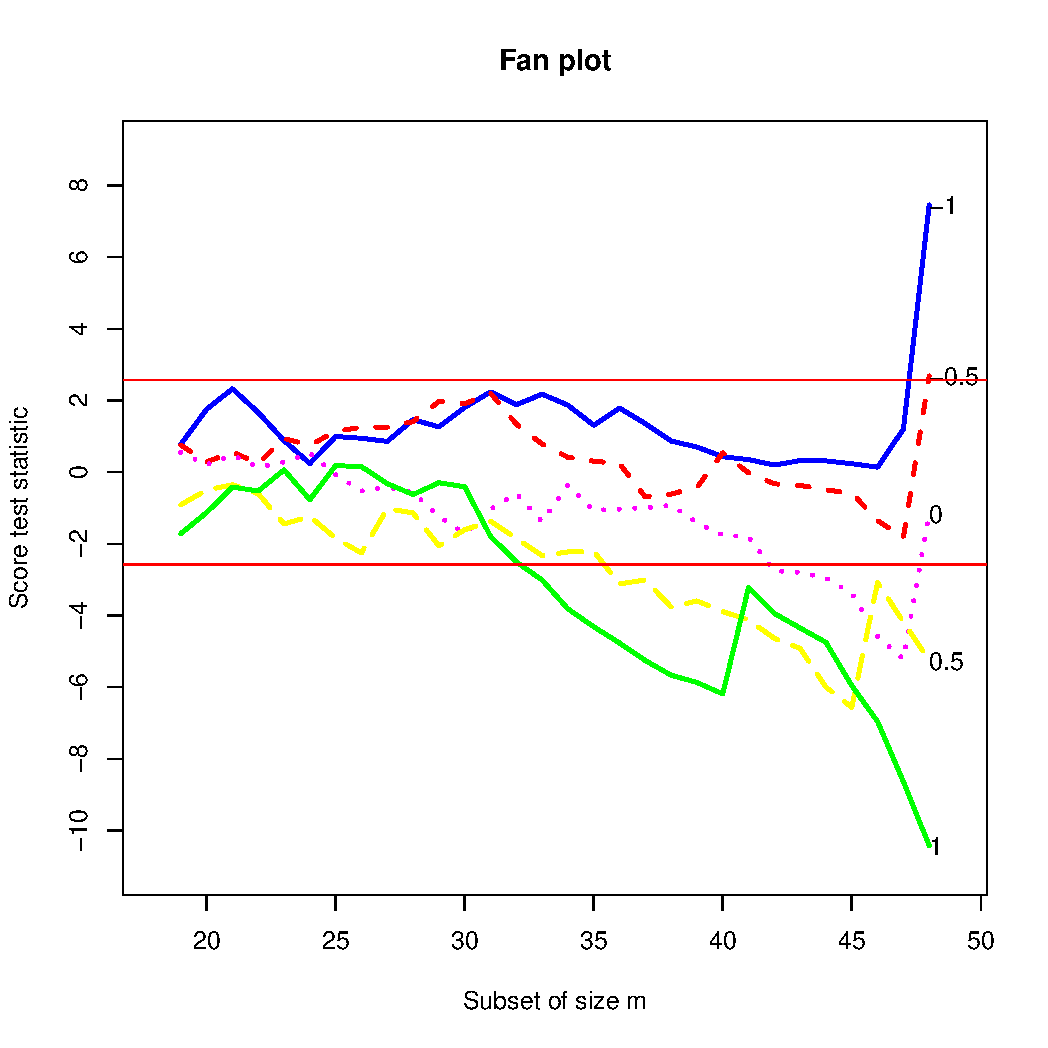
\includegraphics[width=0.8\textwidth]{transreg-ex-2}
\caption{Fan plot for the modified \code{poison} data (one observation changed).}
\label{fig:ex-2}
\end{figure}
\end{center}

At the end of the forward search, the final acceptable value of $\lambda$ 0, with -0.5 on the boundary of the acceptance region. But, much more importantly, Figure~\ref{fig:ex-2} clearly reveals the altered observation and the different effect it has on the five searches. Initially the curves are the same as those of previous Figure~\ref{fig:ex-1}. But for $\lambda=1$ there is a jump due to the introduction of the outlier when\code{m=41} (85\% of the data), which provides evidence for higher values of $\lambda$. For other values of $\lambda$ the outlier is included later in the search. When $\lambda=0.5$ the outlier comes in at\code{m=46}, giving a jump to the score statistic in favor of this value of $\lambda$. For the other values of $\lambda$ the outlier is the last observation to be included. The inclusion of the outlier has  largest effect on the inverse transformation. It is clear from Figure~\ref{fig:ex-2} how this one observation is causing a significant change in the evidence for a transformation.

\subsection[Example 3: Modified poison data (two modified observations)]{Example 3: Modified \code{poison} data (two modified observations)}

The simplest example of masking is when one outlier hides the effect of another, so that neither of them is evident, even when single deletion diagnostics are used. As an example we further modify the poison data. In addition to the previous modification, we also change observation 38 (Poison I, group D) from 0.71 to 0.14. The fan plot shown in the next Figure~\ref{fig:ex-3} clearly shows the effect of the two outliers.

\begin{Schunk}
\begin{Sinput}
> ##  Example 3: modified poison data (change y[8] from 0.23 to 0.13
> ##  and y[38] from 0.71 to 0.14)
> library(fsdaR)
> data(poison)
> poison$Y[8] <- 0.13
> poison$Y[38] <- 0.14
> out3 <- fsrfan(Y~.-1, data=poison)
> plot(out3, ylim=c(-8, 11))
\end{Sinput}
\end{Schunk}

\begin{center}
\begin{figure}[H]
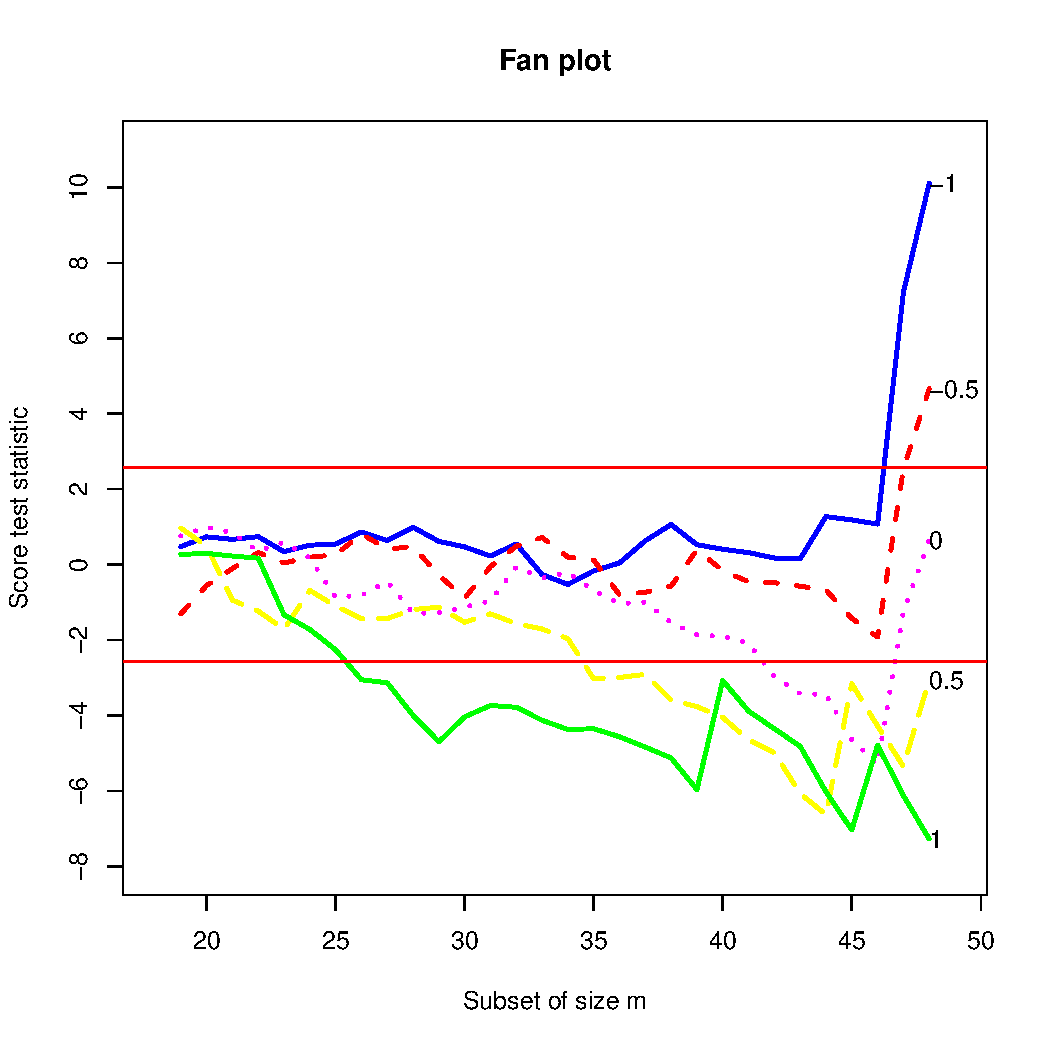
\includegraphics[width=0.8\textwidth]{transreg-ex-3}
\caption{Fan plot for the modified \code{poison} data (two observations changed).}
\label{fig:ex-3}
\end{figure}
\end{center}

The plot also reveals the different effect the two altered observations have on the five searches. Initially the curves are similar to those of the original data shown in Figure~\ref{fig:ex-1}. The difference is greatest for $\lambda=-1$ where the addition of the two outliers at the end of the search causes the statistic to jump from an acceptable value of 1.08 to 10.11. The effect is similar, although smaller, for $\lambda=-0.5$. The most interesting, however, is the log transformation. Towards the end of the search the test statistic is trending downwards, below the acceptable region. But the addition of the last two observations causes a jump in the value of the statistic to a non significant value. The incorrect log transformation is now acceptable. For these three values of $\lambda$ the outliers are the last two observations to be included in the search. They were created by introducing values that are too near to zero when compared with the model fitted to the rest of the data. For the log transformation, and more so for the reciprocal, such values become extreme and so have an appreciable effect on the fitted model. For the other values of $\lambda$ the outliers are included earlier in the search. The effect is most clearly seen when $\lambda=1$; the outliers come in at `\code{m=40} and \code{m=46}, giving upward jumps to the score statistic in favor of this value of $\lambda$. For the last value of \code{la=0.5} one of the outliers is the last value to be included.

\subsection[Example 4: Modified poison data (several modified observations)]{Example 4: Modified \code{poison} data (several modified observations)}

We now create four artificial outliers as shown in Table~\ref{tab:ex-4} below.

\begin{table}[ht]
\centering
\begin{tabular}{crr}
  \hline
 Observation& Original & Modified \\
  \hline
   6 & 0.29 & 0.14 \\
   9 & 0.22 & 0.08 \\
  10 & 0.21 & 0.07 \\
  11 & 0.18 & 0.06 \\
   \hline
\end{tabular}
\caption{The four artificially modified observations.}
\label{tab:ex-4}
\end{table}

The plot shown in Figure~\ref{fig:ex-4} is, indeed, more complicated than the plots for the singly modified data and for the doubly modified data.

\begin{Schunk}
\begin{Sinput}
> ##  Example 4: modified poison data (four observations are changed)
> library(fsdaR)
> data(poison)
> poison$Y[6] <- 0.14
> poison$Y[9] <- 0.08
> poison$Y[10] <- 0.07
> poison$Y[11] <- 0.06
> out4 <- fsrfan(Y~.-1, data=poison, init=10)
> plot(out4, ylim=c(-10, 22))
\end{Sinput}
\end{Schunk}

\begin{center}
\begin{figure}[H]
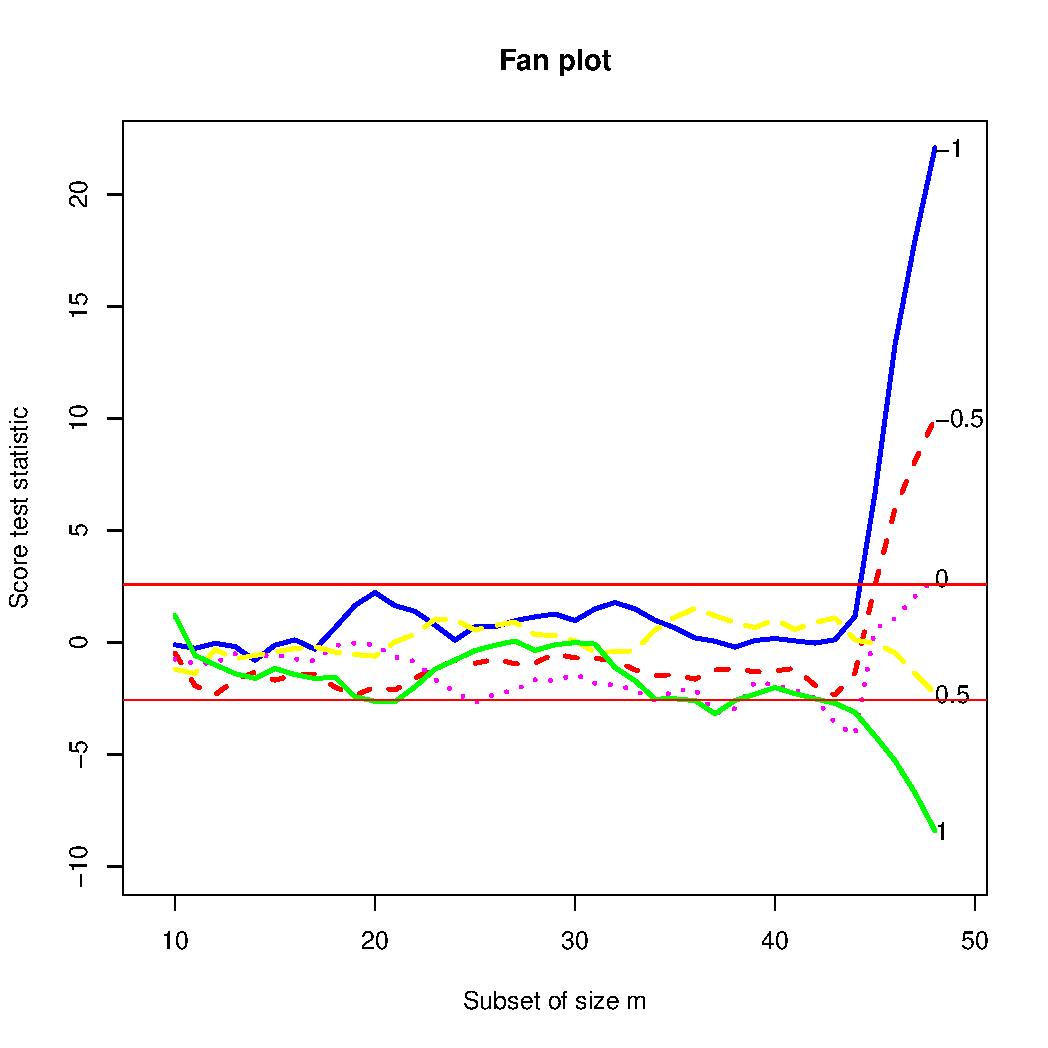
\includegraphics[width=0.8\textwidth]{transreg-ex-4}
\caption{Fan plot for the modified \code{poison} data (four observations changed).}
\label{fig:ex-4}
\end{figure}
\end{center}

Some curves are within the bounds for most of the subsets and then increase rapidly at the end; others go outside the 1\% boundary, only to return at the end. Both ways are associated with influential observations. For $\lambda=-1$ the curve lies well within the boundary, with no particular pattern, until $m=45$. The addition of the last four observations, which are the four outliers, causes a rapid increase in the value of the score test from 1.16 to 22.1 and provides strong evidence against $\lambda=-1$. It is interesting that the observations included in this search when \code{m=44} is number 8, the last to be included for the original data and this value of $\lambda$. The behavior of the curve for $\lambda=-0.5$ is similar, but much less extreme. The four outliers are again included at the end, causing the statistic to increase from -1.36 to 10.0. The curve for $\lambda=0$ first goes below the boundary but the inclusion of the four contaminated observations, again in the last four steps of the forward search, brings it above the upper threshold. The statistic for $\lambda=0.5$ spends much more of the central part of the search outside the lower boundary. As we have seen, the final value of $Tp(0.5)$ is -2.29. But for values of $m$ between 22 and 37 the curve lies approximately on or below the boundary. The inclusion of units 9, 10 and 11 at \code{m=38}, 39 and 40 increases the value of the score statistic from -2.65 to 1.89. From this step on wards the curve decreases monotonically, except at \code{m=43} when unit 6 is included, the first modified unit to be included. It is interesting that, in this scale, the four contaminated observations are not extreme and so do not enter in the last steps of the forward search. But the forward plot enables us to detect their effect on the score statistic. The indication of this plot is that one possible model for these data takes $\lambda=-1$ for the greater part of the data, with four outliers. To confirm this suggestion we look at the plot that monitors the scaled residuals during the forward search. This is shown, for $\lambda=-1$ in Figure 5 below. This plot, obtained with the following code, beautifully indicates the structure of the data. On this scale there are the four outliers, observations 6, 9, 10 and 11, which enter in the last four steps of the forward search.


\begin{Schunk}
\begin{Sinput}
> ##  Example 4a: modified poison data (four observations
> ##  are changed) with the reciprocal transformation
> poison$Y <- poison$Y ^ (-1)
> set.seed(1234)
> out4a <- fsreg(Y~.-1, data=poison, method="LMS", msg=FALSE)
> out4a <- fsreg(Y~.-1, data=poison, monitoring=TRUE,
+           lms=out4a.bs, msg=FALSE)
> ##  Monitoring the scaled residuals: a label is written
> ##  for the residuals greater than 2
> resfwdplot(out4a, fg.thresh=2)
\end{Sinput}
\end{Schunk}

\begin{center}
\begin{figure}[H]
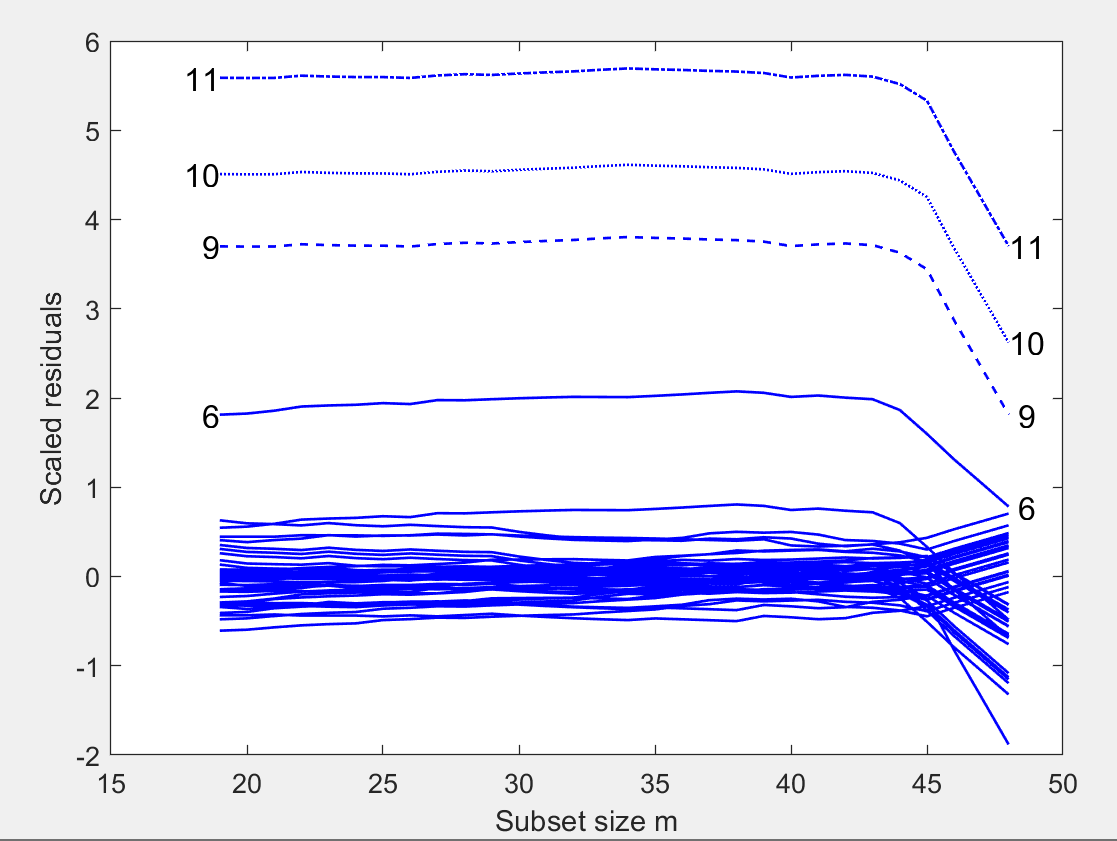
\includegraphics[width=0.8\textwidth]{transreg-ex-4a.png}
\caption{Residual forward plot for the modified \code{poison} data (four observations changed) with the reciprocal transformation.}
\label{fig:ex-4a}
\end{figure}
\end{center}


Similarly, if we run the automatic outlier detection procedure in \code{fsreg()} using the following code, we can clearly spot the 4 outliers.

\begin{Schunk}
\begin{Sinput}
> ##  Example 4b: automatic outlier detection for the
> ##  modified poison data (four observations are changed)
> ##  with the reciprocal transformation
> 
> set.seed(1234)
> out4b <- fsreg(Y~.-1, data=poison, control=FSR_control(plot=2, msg=FALSE))
\end{Sinput}
\end{Schunk}

\begin{center}
\begin{figure}[H]
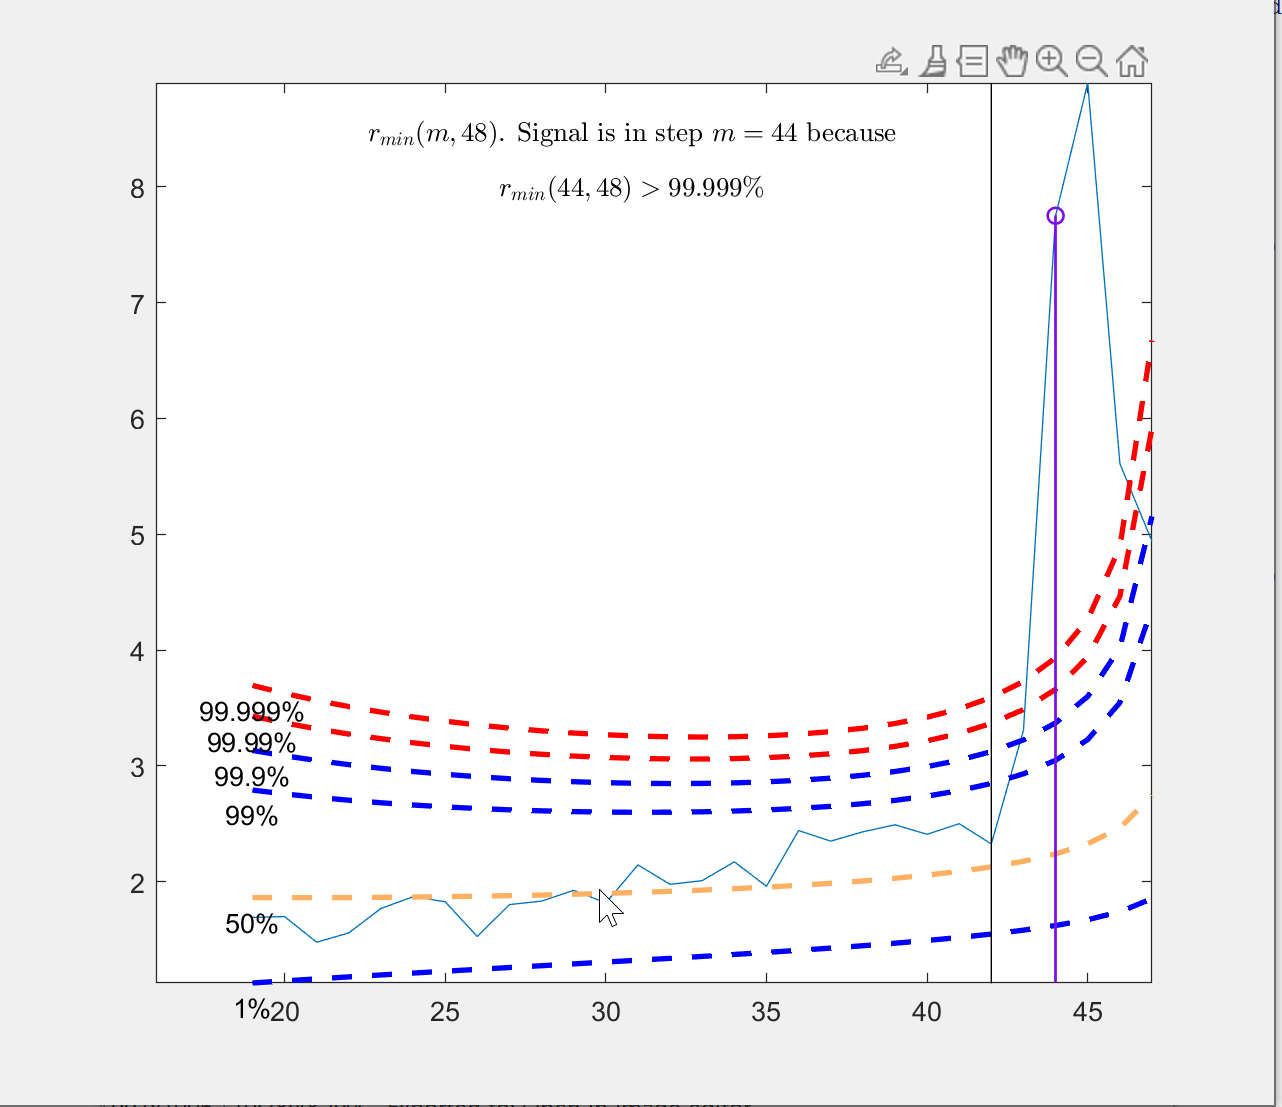
\includegraphics[width=0.4\textwidth]{transreg-ex-4b-1.png}
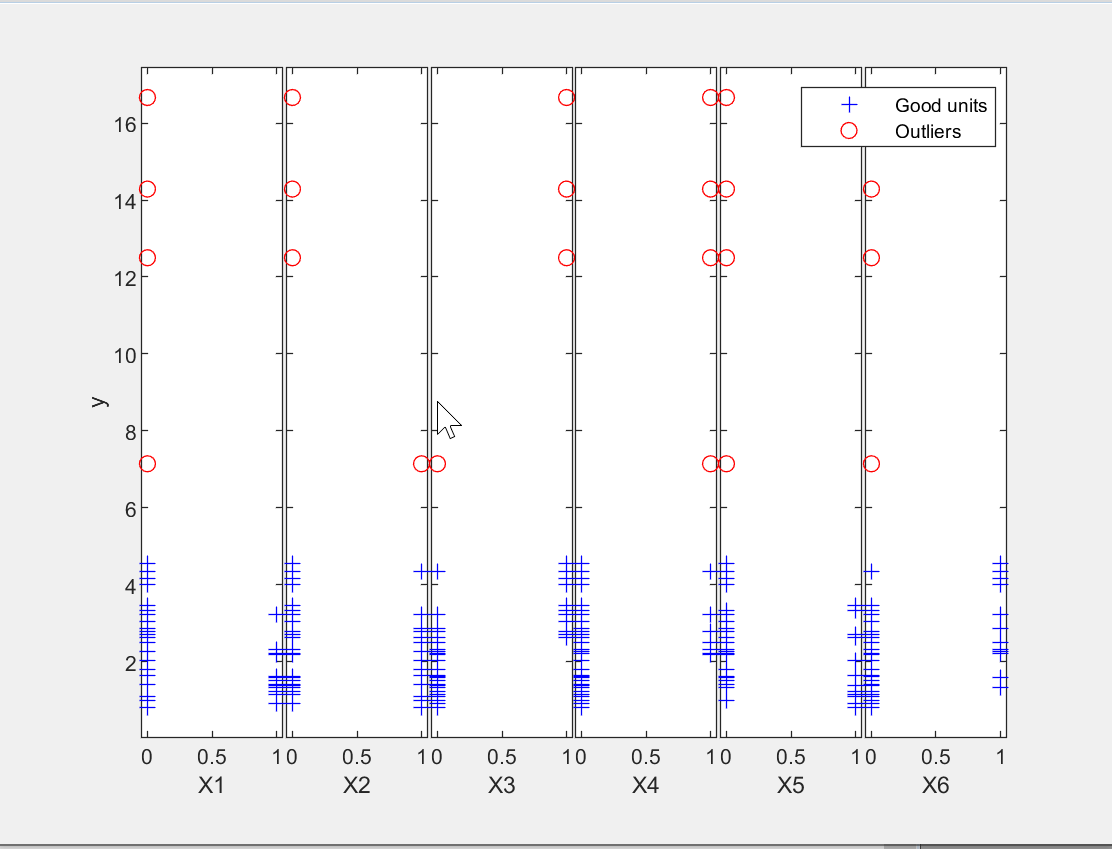
\includegraphics[width=0.45\textwidth]{transreg-ex-4b-2.png}
\caption{Automatic outlier detection for the modified \code{poison} data (four observations changed) with the reciprocal transformation.}
\label{fig:ex-4b-1}
\end{figure}
\end{center}

\begin{center}
\begin{figure}[H]
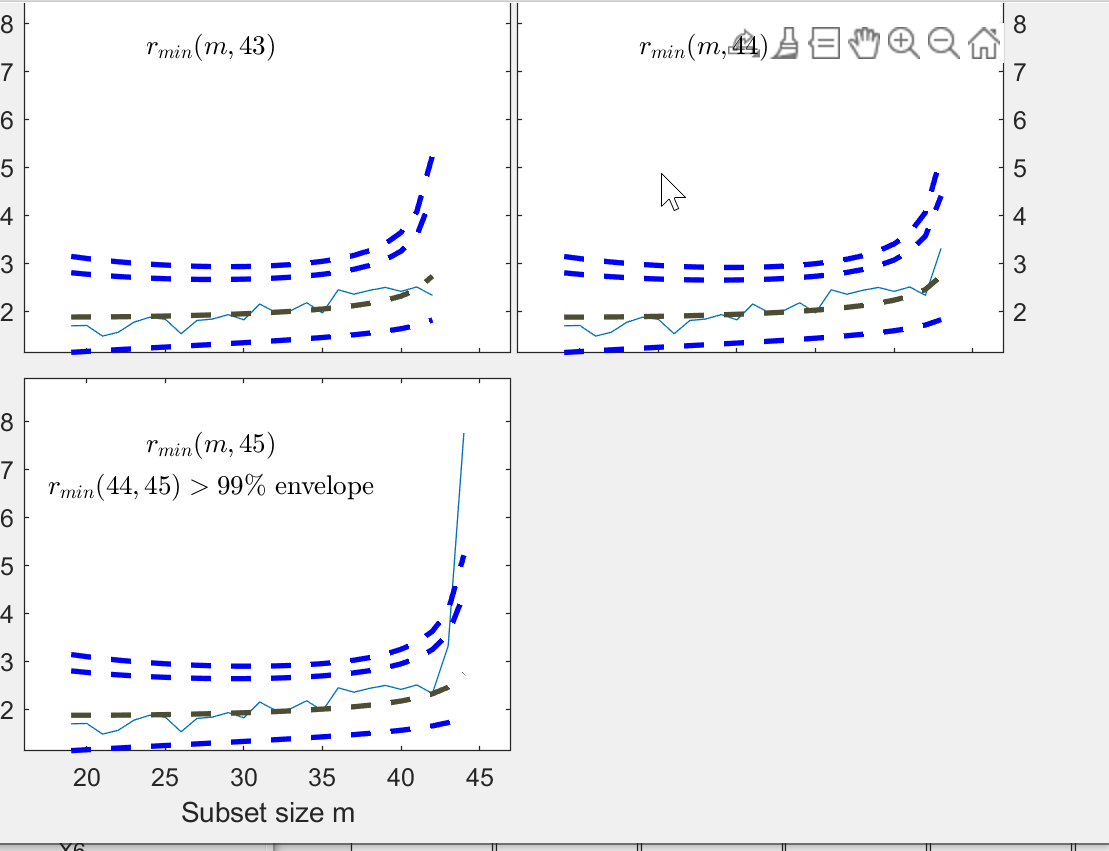
\includegraphics[width=0.8\textwidth]{transreg-ex-4b-3.png}
\caption{Automatic outlier detection for the modified \code{poison} data (four observations changed) with the reciprocal transformation (Cont.).}
\label{fig:ex-4b-2}
\end{figure}
\end{center}

\bibliography{references}
\end{document}
